\subsection{Simulation}
A solution with an input data generator and an output error checker has been adopted for the simulation of the circuit. A python script has been used to generate a sine waveform, which is processed in parallel by the designed circuit and the ideal model described in C. The output results are written on two files that are processed by an additional python script that computes the error as the difference between the output of the DUT and the C model.
In \autoref{fig:wave_start} is shown the wave with DUT signals. Note that when the $VIN$ signal becomes valid the circuit starts to sample the input data and after a latency of 2 clock periods the results are ready to output, so the $VOUT$ signal is asserted.

\begin{figure}[h]
	\center
	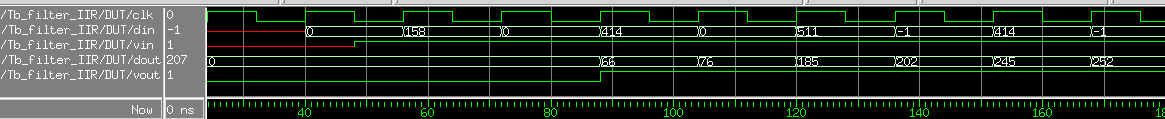
\includegraphics[width=1\textwidth]{wave_start.png}
	\caption{Start of the simulation}
	\label{fig:wave_start}
\end{figure}

In \autoref{fig:wave_vin} the correct functioning can be noticed even when $VIN$ is negated, in fact the data at the output of the filter, $d\_out$, remain unchanged when this situation occurs because the circuit stops sampling the input data. When $VIN$ returns to 1, after a latency of 1 clock period, the output data changes again.

\begin{figure}[h]
	\center
	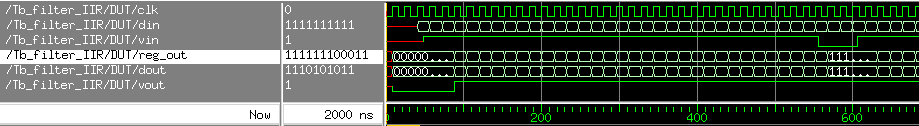
\includegraphics[width=1\textwidth]{wave_vin_0_1.png}
	\caption{Simulation of the $VIN$ signal transition}
	\label{fig:wave_vin}
\end{figure}

After verification of the correct timing of the circuit, the numerical results produced were checked. In \autoref{tab:tab_results} is shown an extract of the output data from the ideal model and the circuit designed with the same set of input data. It is noticeable that there is a perfect equality of results that confirms the correct operation of the designed filter.

\begin{table}[h]
\begin{center}
\begin{tabular}{|l|l|l|l|}
\hline
Input & DUT output & C model output & Error \\
\hline
511 & 252 & 252 & 0 \\
-1 & 213 & 252 & 0 \\
414 & 207 & 207 & 0 \\
-1 & 98 & 98 & 0 \\
158 & 80 & 80 & 0 \\
-1 & -56 & -56 & 0 \\
-159 & -77 & -77 & 0 \\
-1 & -188 & -188 & 0 \\
-415 & -206 & -206 & 0 \\
-1 & -250 & -250 & 0 \\
\hline
\end{tabular}
\end{center}
\caption{Results of the simulation}
\label{tab:tab_results}
\end{table}